\documentclass[12pt,a4paper]{article}

\usepackage[T1]{fontenc}
\usepackage[utf8]{inputenc}
\usepackage[polish]{babel}
\usepackage{indentfirst}
\usepackage{amsfonts}
\usepackage{amsmath}
\usepackage{algorithmic}

\usepackage[margin=0.5in,headheight=48pt,top=78pt]{geometry}
\frenchspacing
\setlength{\parskip}{1em}
\setlength{\parindent}{0em}
\def\N{\mathbb{N}}
\def\R{\mathbb{R}}
\newcommand{\zadanie}[1]{\par\textbf{Zadanie #1}}
\newcommand{\odp}[1]{\textbf{Odpowiedź:} #1}


\usepackage{tikz}

\usepackage{fancyhdr}
\pagestyle{fancy}
\fancyhf{} % clear all fields
\fancyhead[C]{ \textbf{AISD} - Lista 4 Zadanie 1\\ Wiktor Pilarczyk}

\begin{document}
\section{Algorytm}
Algorytm jest prawie identyczny do algorytmu przedstawionego na wykładzie tylko dla każdej kolumny mamy dodatkowo dwie pętle, które sprawdzają ruchy w góre i w dół, a przy odzyskiwaniu wyniku mamy dodatkowe dwa przypadik ruchów.
\begin{figure}[!htb]
\centering
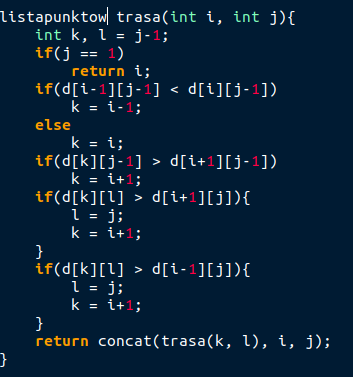
\includegraphics[width=6cm,height=6cm]{algo.png}
\caption{echo reply}
\end{figure}
\begin{figure}[!htb]
\centering
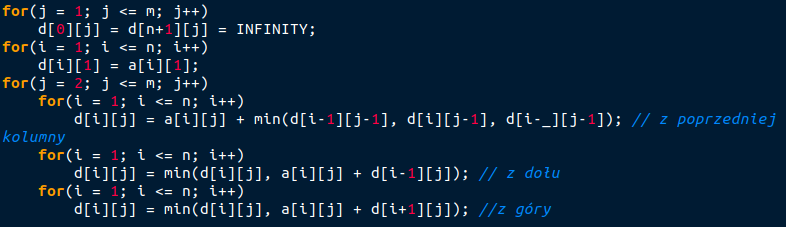
\includegraphics[width=11cm,height=5cm]{sciezka.png}
\caption{echo reply}
\end{figure}
\section{Dowód poprawności}
Załóżmy nie wprost, że otrzymaliśmy nie optymalną ścieżkę więc nasz wynik jest większy niż optymalny.To oznacza, że punkt, w którym się kończy optymalna ścieżka ma u nas większy koszt dojścia, wybierzmy pierwszy taki punkt, w którym koszt dojścia do tego pola jest większy niż w ścieżce optymalnej. Skoro poprzednik ma obliczony dobry koszt oznacza, że nie rozpatrzyliśmy przypadku dojścia do tego elementu (nieoptymalnego) po obliczeniu kosztu dojścia do poprzednika. Rozważmy przypadki gdzie leży poprzedni element:


1. Jeśli poprzedni element leży w innej kolumnie (z mniejszym indeksem) na pewno rozważyliśmy taki przypadek, ponieważ po przejściu do następnej kolumny nie zmieniamy już wyniku w poprzednich kolumnach. Więc mamy sprzeczność \\

2. Podobnie przy elemencie z "dołu", ponieważ jest to ostatnia pętla.

3. Poprzedni element leży powyżej nas, mogliśmy zmienić jego wartość przy sprawdzaniu czy nie ma lepszej drogi przychodząc z dołu, ale z prostej obserwacji można zauważyć, że jeśli byśmy zaktualizowali element, który jest powyżej to oznacza, że nasza wartość jest mniejsza bądź równa wartości powyżej (wagi są nieujemne), więc nie jesteśmy w stanie otrzymać lepszego wyniku w tym punkcie. Otrzymujemy sprzeczność.

\section{Złożoność}
Obliczanie tablicy najmniejszego kosztu dojścia do pola X wynosi $\Theta(n*m)$ ponieważ dla każdej kolumny (m) wykonujemy n*3 obliczeń. Koszt odzyskiwania trasy nie ma większej złożoności niż $\Theta(n*m)$, ponieważ jak wcześniej pokazaliśmy nic nie zyskujemy przechodząc wielokrotnie jakieś pole. Więc złożoność naszego algorytmu to $\Theta(n*m)$.

\end{document}

